\documentclass[12pt,a4paper]{report}

\usepackage{anysize}
\usepackage{listings}
\usepackage{amsmath}
\usepackage{siunitx}
\usepackage{hyperref}
\usepackage{circuitikz}
\usetikzlibrary{positioning}
\usepackage{float}
\usepackage{epstopdf}

\lstset{
	backgroundcolor=\color[rgb]{0.95,0.95,0.95},
	basicstyle=\scriptsize\ttfamily,
	breakatwhitespace=false,
	breaklines=true,
	frame=single,
	rulecolor=\color[rgb]{0,0,0},
	keepspaces=true,
	showstringspaces=false,
	showtabs=false,
	tabsize=2,
	aboveskip=3pt,
	belowskip=3pt,
	columns=fixed,
	numbers=left,
	numbersep=5pt,
	numberstyle=\tiny\color[rgb]{0.5,0.5,0.5},
	stepnumber=1
}

\lstdefinestyle{MATLAB_CODE}{
	language=Matlab,
	keywordstyle=\color[rgb]{0,0,1},
	commentstyle=\color[rgb]{0,0.6,0},
	stringstyle=\color[rgb]{0.58,0,0.82},
	deletekeywords={},
	morekeywords={nchoosek}
}

\pagestyle{empty}
\marginsize{20mm}{20mm}{20mm}{20mm}

\begin{document}

\begin{center}

	{\huge Alkatr\'{e}sztoleranci\'{a}k hat\'{a}s\'{a}nak vizsg\'{a}lata}
	
	\vspace{5mm}
	
	\begin{circuitikz}[on grid]
		\node(ube)[label=left:$U_\mathrm{be}$]{};
		\node(phi1)[right=2 of ube][label=below:$\varphi$]{};
		\node(phi2)[right=2 of phi1][label=above:$U_\mathrm{ki}$]{};
		\node[ground](gnd)[below=2 of phi2]{};
		\node[op amp](opamp)[right=2 of phi2, yshift=-5mm, yscale=-1]{};
		\node(uki)[right=0.6 of opamp.out][label=right:$U_\mathrm{ki}$]{};
		\node(c1)[above=1.2 of phi1]{};
		\draw(ube)to[R=$R_1$,o-](phi1)
		to[R=$R_2$](phi2)
		to[short](opamp.+);
		\draw(phi1)to[short,*-](c1)
		to[C=$C_1$](c1 -| opamp.out)
		to[short,-*](opamp.out);
		\draw(phi2)to[C, l_=$C_2$,*-](gnd);
		\draw(opamp.out)to[short,-o](uki);
		\draw(opamp.out)to[short,*-]+(0, -1.35)
		to[short]+(0,0) -| (opamp.-);
	\end{circuitikz}

\end{center}

\noindent N\'{e}vleges alkatr\'{e}sz\'{e}rt\'{e}kek \'{e}s worst-case toleranci\'{a}k:
\begin{align*}
	R_1&=\SI{10}{\kilo\ohm}  \pm 1\% \\
	R_2&=\SI{10}{\kilo\ohm}  \pm 1\% \\
	C_1&=\SI{1}{\nano\farad} \pm 5\% \\
	C_2&=\SI{2}{\nano\farad} \pm 5\% 
\end{align*}

\noindent Csom\'{o}ponti egyenletek:
\begin{align*}
	&\frac{\varphi-U_\mathrm{be}}{R_1}+\frac{\varphi-U_\mathrm{ki}}{R_2}+\frac{\varphi-U_\mathrm{ki}}{\frac{1}{j\omega C_1}}=0 \\[6pt]
	&\frac{U_\mathrm{ki}-\varphi}{R_2}+\frac{U_\mathrm{ki}-0}{\frac{1}{j\omega C_2}}=0
\end{align*}

\noindent A megold\'{a}s m\'{a}trixos alakban:
\begin{align*}
	\begin{pmatrix}
		\varphi \\[6pt]
		U_\mathrm{ki}
	\end{pmatrix}
	=
	\begin{pmatrix}
		\frac{1}{R_1}+\frac{1}{R_2}+j\omega C_1 & -\frac{1}{R_2}-j\omega C_1 \\[6pt]
		-\frac{1}{R_2} & \frac{1}{R_2}+j\omega C_2
	\end{pmatrix}^{-1}
	\begin{pmatrix}
		\frac{U_\mathrm{be}}{R_1} \\[6pt]
		0
	\end{pmatrix}
\end{align*}

\clearpage

{\centering\huge MATLAB k\'{o}d\\}

\vspace{5mm}

\lstset{style=MATLAB_CODE}
\begin{lstlisting}
%% parameterek
f=10:10:100e3; % frekvencia sweep [Hz]
Ube=1;         % gerjesztes komplex amplitudoja [V]
N=4;           % alkatreszek szama
R1n=10e3; R1tol=0.01;
R2n=10e3; R2tol=0.01;
C1n=1e-9; C1tol=0.05;
C2n=2e-9; C2tol=0.05;

%% szimulacio
Uki=zeros(length(f),3);
for ii=1:length(f)
    for jj=1:2^N+1
        if jj==2^N+1
            R1=R1n;
            R2=R2n;
            C1=C1n;
            C2=C2n;
        else
            tols=2*de2bi(jj-1,N)-1;
            R1=R1n*(1+tols(1)*R1tol);
            R2=R2n*(1+tols(2)*R2tol);
            C1=C1n*(1+tols(3)*C1tol);
            C2=C2n*(1+tols(4)*C2tol);
        end
        omega=2*pi*f(ii);
        A=[1/R1+1/R2+1j*omega*C1  ,  -1/R2-1j*omega*C1  ;
           -1/R2                  ,   1/R2+1j*omega*C2 ];
        B=[Ube/R1 ; 0];
        x=A\B;
        if jj==1
            Uki(ii,1)=x(2);
            Uki(ii,3)=x(2);
        elseif jj==17
            Uki(ii,2)=x(2);
        elseif abs(x(2))<abs(Uki(ii,1))
            Uki(ii,1)=x(2);
        elseif abs(x(2))>abs(Uki(ii,3))
            Uki(ii,3)=x(2);
        end
    end
end

%% abrazolas
figure(1);
mag=abs(Uki);
subplot(211);
fill([f f(end:-1:1)],[mag(:,3)' mag(end:-1:1,1)'],[0.59 0.59 0.78],'LineStyle','none');
hold on;
h=plot(f,mag);
hold off;
set(gca,'XScale','log','XGrid','on','YGrid','on');
set(h,{'color'},{'k';'r';'k'});
xlabel('f [Hz]');
ylabel('|H(f)|');
subplot(212);
phase=unwrap(angle(Uki))*180/pi;
fill([f f(end:-1:1)],[phase(:,3)' phase(end:-1:1,1)'],[0.59 0.59 0.78],'LineStyle','none');
hold on;
h=plot(f,phase);
hold off;
set(gca,'XScale','log','XGrid','on','YGrid','on');
set(h,{'color'},{'k';'r';'k'});
xlabel('f [Hz]');
ylabel('\phi(f) [\circ]');
\end{lstlisting}

\clearpage

{\centering\huge Kimenet\\}

\begin{figure}[H]
	\centering
	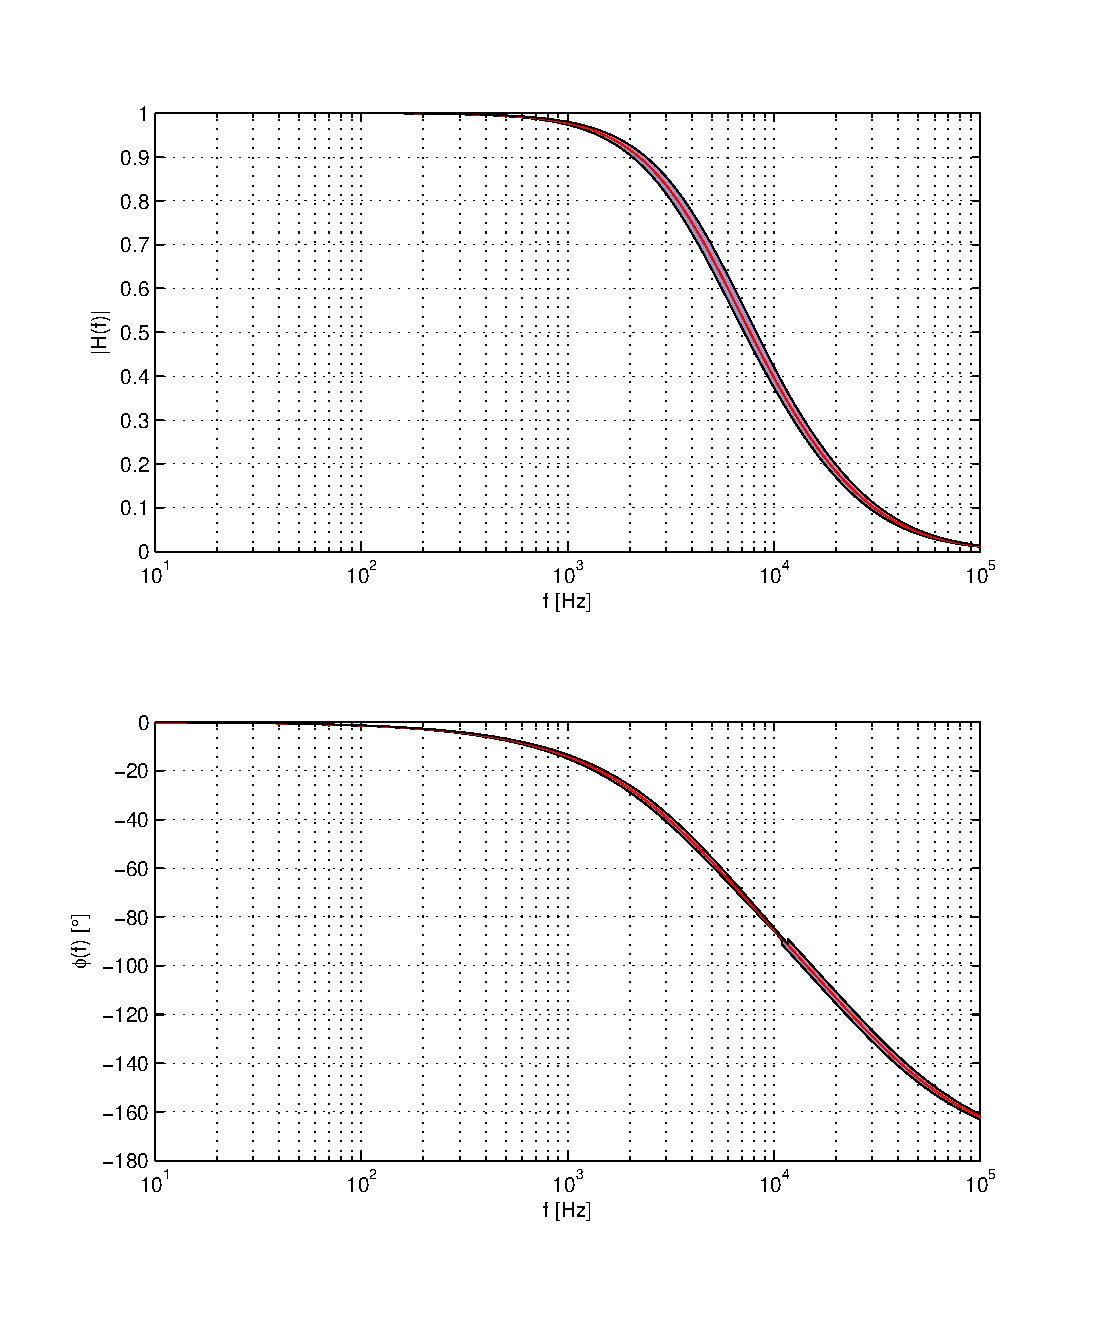
\includegraphics{output.eps}
\end{figure}

\clearpage

{\centering\huge LTspice szimul\'{a}ci\'{o}\\}

\begin{figure}[H]
	\centering
	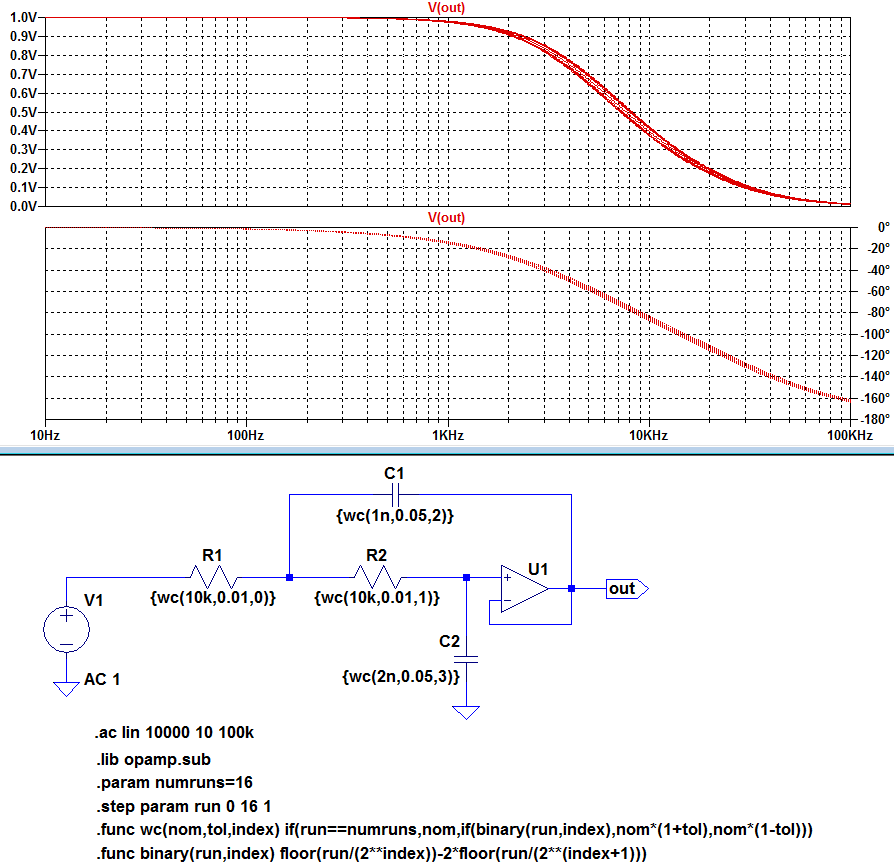
\includegraphics[scale=0.5]{ltspice.png}
\end{figure}


\end{document}